\section{Optimization Methods}

In this section I will present a few optimization algorithms.

\subsection{Line Search Methods}

The \textit{line search} is a strategy that selects the step size (commonly represented by $t$) that determines where along the line $\left\lbrace x+t\Delta x\mid t\in\mathbb{R}_+\right\rbrace$ the next iterate in the descent method will be. ($\Delta x$ represents the \textit{descent direction}, .) Line search strategies can either be \textit{exact} or \textit{inexact}.

\subsubsection*{Exact Line Search}

An \textit{exact line search} chooses the value $t$ along the ray $\left\lbrace x+t\Delta x\mid t\in\mathbb{R}_+\right\rbrace$ that exactly minimizes the function of interest $f$:
$$t=\arg\min_{s\geq 0}f(x+s\Delta x)$$
An exact line search is almost never practical. In very special cases, such as some quadratic optimization problems, where computing the cost of the minimization problem is low compared to actually calculating the search direction, one might employ an exact line search.

\subsubsection*{Backtracking Line Search}
Most often in practice we use \textit{inexact line searches}. In an inexact line search, we choose $t$ such that $f$ is \textit{approximately} minimized or reduced ``enough'' along $\left\lbrace x+t\Delta x\mid t\in\mathbb{R}_+\right\rbrace$.

One inexact line search strategy is the \textit{Backtracking Line Search}.
\begin{algorithm}[H]
	\caption{Backtracking Line Search \cite[]{Boyd2004}\label{BacktrackingLineSearchAlg}}
	\begin{algorithmic} 
		\State \textbf{given} a descent direction $\Delta x$ for $f$ at $x\in\textbf{dom}f,\alpha\in(0,0.5),\beta\in(0,1)$.
		\State $t:=1$.
		\While{$f(x+t\Delta x)>f(x)+\alpha t\nabla f(x)^T\Delta x$}
		\State $t:=\beta t$
		\EndWhile
	\end{algorithmic}
\end{algorithm}

``Backtracking'' in the name is refers to the fact that the method starts with a unit step size $(t=1)$ and then reduces the step size (``backtracks'') by the factor $\beta$ until we meet the stopping criterion $f(x+t\Delta x)\leq f(x)+\alpha t\nabla f(x)^T\Delta x$.

%%% Need to reproduce image on own or something for final draft...

Figure 9.1 \cite[p. 465]{Boyd2004} demonstrates the Backtracking Line Search visually for a parabola.
\begin{center}
	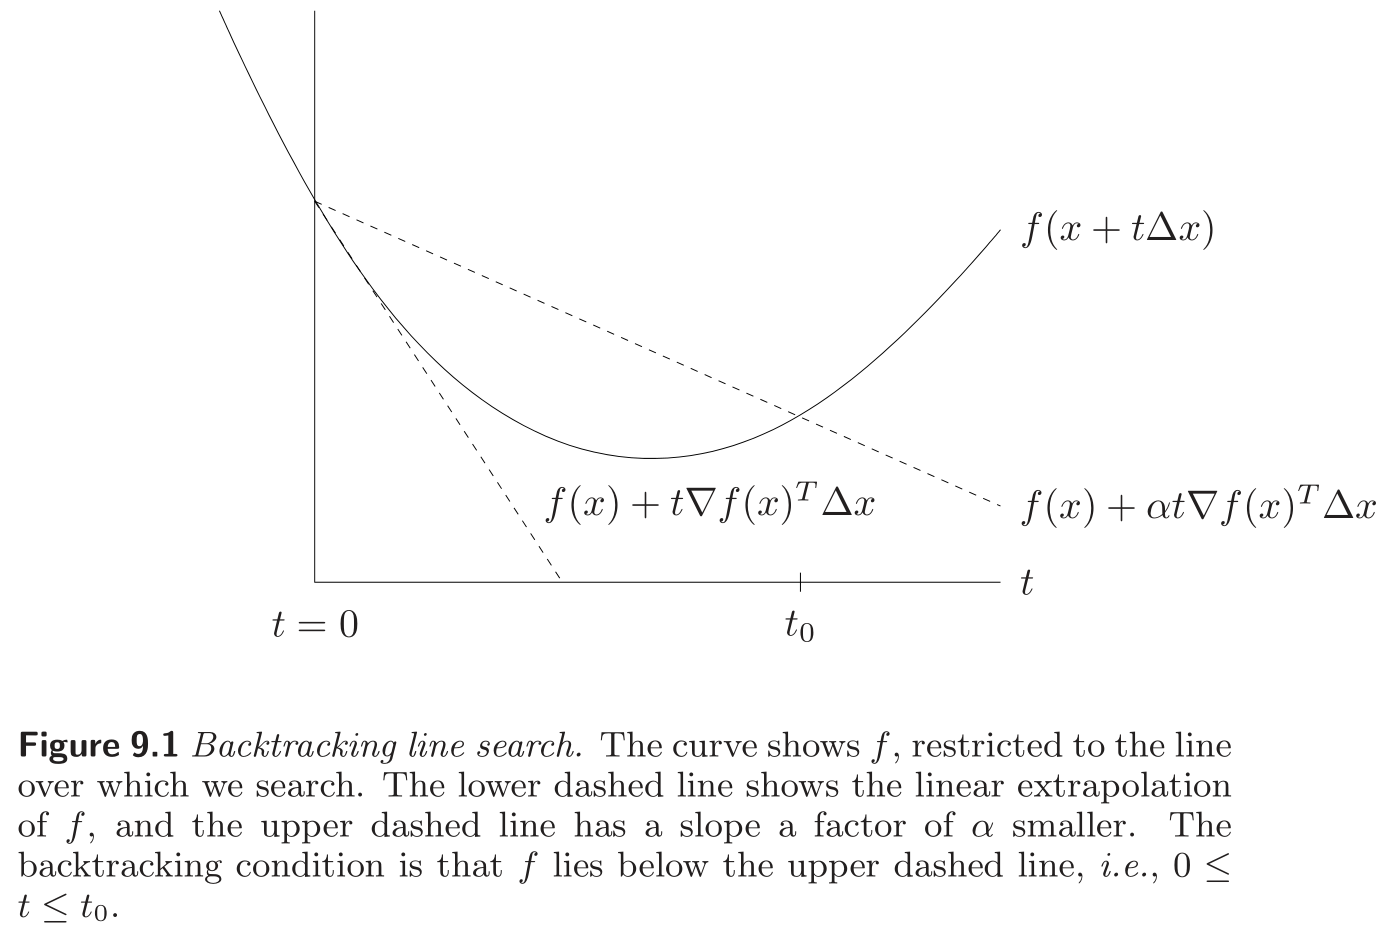
\includegraphics[width=0.75\textwidth]{Chapter_I_Background/Images/backtracking_line_search_diagram.png}
\end{center}

Notice that the backtracking search will find a step size $t$ such that $0\leq t\leq t_0$ and that for such $t$, $f(x+t\Delta x)$ is smaller relative to $f(x)$. However, the step size we choose may not exactly be the minimum of the function, but we have funneled it down to be closer to the minimum of $f$.
\subsection{Gradient Descent}

The gradient descent method chooses the search direction to be the negative gradient. That is, in this method we set $\Delta x=-\nabla f(x)$, where $f$ is the function we seek to optimize. Since the gradient of a function gives the direction of greatest increase, naturally the negative gradient will give the direction of the most rapid decline.

\begin{algorithm}
	\caption{Gradient Descent Method \cite[]{Boyd2004}\label{GradientDescentAlg}}
	\begin{algorithmic} 
		\State \textbf{given} a starting point $x\in\textbf{dom}f$.
		\Repeat
		\begin{enumerate}
			\item $\Delta x:=-\nabla f(x)$.
			\item \textit{Line search.} Choose step size $t$ via exact or backtracking line search.
			\item \textit{Update.} $x:=x+t\Delta x$.
		\end{enumerate}
		\Until{stopping criterion is satisfied.}
	\end{algorithmic}
\end{algorithm}

Notice in Algorithm \ref{GradientDescentAlg} that essentially a line search is used to determine a step size and then we update our iterate in the direction of the steepest descent. This is repeated until we meet some sort of stopping criterion, typically something of the form $\|\nabla f(x)\|_2\leq\eta$, where $\eta$ is small and positive. Another common stopping criterion is to stop the algorithm when no significant progress is made between iterates by stopping the algorithm when $\|f_{k+1}-f_{k}\|<\eta$.

An implementation of the gradient descent algorithm in the Julia language can be found in the appendix.

\subsection{Nonlinear Conjugate Gradient}

The Nonlinear Conjugate Gradient method works similarly to the gradient descent algorithm, but adds the additional requirement that in each iteration gradient is orthogonal to each previous search direction.

Suppose we have a function $f(x)$ of $N$ variables. Let $x_0$ be an initial guess value for the minimum. The opposite of the gradient will give the direction of steepest descent. Therefore, we start off by setting $\Delta x_0=-\nabla f(x_0)$.

We set an adjustable step length $\alpha$ and perform a line search in the direction $d_0=\Delta x_0$ until a minimum of $f$ is reached:
\begin{align*}
	&\alpha_0:=\arg\min_{\alpha} f(x_0+\alpha\Delta x_0),\\
	&x_1=x_0+\alpha_0\Delta x_0.
\end{align*}

Suppose we were to simply iterate this process and for each step $i$ we do the following:

\begin{enumerate}
	\item Set $\Delta x_i=-\nabla f(x_i)$
	\item Calculate $\alpha_i=\arg\underset{\alpha}{\min}\ f(x_i+\alpha\Delta x_i)$
	\item Compute $x_{i+1}=x_i+\alpha_i\Delta x_i$
\end{enumerate}

However, there is an issue with this proposed iterative scheme: We have moved $\alpha_i$ in direction $\Delta x_i$ to find the minimum value in that direction, but by moving $\alpha_{i+1}$ in direction $\Delta x_{i+1}$ we may have accidentally \textit{undone} the progress made in the previous iteration so that we no longer have a minimum value in direction $\Delta x_i$. We can fix this problem by making sure that successive direction vectors have no influence in the directions of previous iterations. That is, we require our directions in each iteration to be conjugate (with respect to the matrix of coefficient for our system) to one another. Therefore, rather than taking $\Delta x_{i+1}$ to be $-\nabla f(x_i)$, we compute a direction conjugate to all previous directions by some pre-chosen methodology. This suggests the following iterative scheme:

After the first iteration, the following steps constitute one iteration along a conjugate direction:
\begin{enumerate}
	\item Calculate the new steepest descent direction: $\Delta x_i=-\nabla f(x_i)$,
	\item Compute $\beta_i$ using some formulation. Two options are below:
	\begin{itemize}
		\item Fletcher--Reeves: $\beta_i^{FR}=\frac{\Delta x_i^T\Delta x_i}{\Delta x_{i-1}^T\Delta x_{i-1}}$
		\item Polak--Ribi\`{e}re: $\beta_{i}^{PR}=\frac{\Delta x_i^T(\Delta x_i-\Delta x_{i-1})}{\Delta x_{i-1}^T\Delta x_{i-1}}$
	\end{itemize}
	\item Update the conjugate direction: $d_i=\Delta x_i+\beta_i d_{i-1}$,
	\item Line search: Optimize $\alpha_i =\arg\underset{\alpha}{\min}\ f(x_i+\alpha d_i)$,
	\item Update iterate value: $x_{i+1}=x_i+\alpha_i d_i$.
\end{enumerate}

Algorithm \ref{CongGradAlg} uses the Newton-Raphson method to find the values of $\alpha_i$.

\begin{algorithm}
	\caption{Nonlinear Conjugate Gradient Using Newton-Raphson \cite[]{Shewchuk1994}\label{CongGradAlg}}
	Given a function $f$, a starting value $x$, a maximum number of CG iterations $i_{\text{max}}$, a CG error tolerance $\epsilon<1$, a maximum number of Newton-Raphson iterations $j_{\text{max}}$, and a Newton-Raphson error tolerance $\varepsilon<1$:
	\begin{algorithmic}
		\State $i\Leftarrow 0$
		\State $k\Leftarrow 0$
		\State $r\Leftarrow -f^{\prime}(x)$
		\State $d\Leftarrow r$
		\State $\delta_{\text{new}}\Leftarrow r^Tr$
		\State $\delta_0\Leftarrow\delta_{\text{new}}$
		\While{$i<i_{\max}$ and $\delta_{\text{new}}>\epsilon^2\delta_0$}
		\State $j\Leftarrow 0$
		\State $\delta_d\Leftarrow d^Td$
		\While{true}
		\State $\alpha\Leftarrow -\frac{\left[f^{\prime}(x)\right]^Td}{d^Tf^{\prime\prime}(x)d}$
		\State $x\Leftarrow x+\alpha d$
		\State $j\Leftarrow j+1$
		\State $j<j_{\text{max}}$ and $\alpha^2\delta_d>\varepsilon^2$ OR \textbf{Break}
		\EndWhile
		\State $r\Leftarrow -f^{\prime}(x)$
		\State $\delta_{\text{old}}\Leftarrow\delta_{\text{new}}$
		\State $\delta_{\text{new}}\Leftarrow r^T r$
		\State $\beta\Leftarrow\frac{\delta_{\text{new}}}{\delta_{\text{old}}}$
		\State $d\Leftarrow r+\beta d$
		\State $k\Leftarrow k+1$
		\If{$k=n$ or $r^T d\leq 0$}
		\State $d\Leftarrow r$
		\State $k\Leftarrow 0$
		\EndIf
		\State $i\Leftarrow i+1$
		\EndWhile
	\end{algorithmic}
\end{algorithm}

To get some intuition of how this algorithm operates, let's look at it applied to a quadratic function.

\paragraph{Example: Rosenbrock Function}